% vim: set textwidth=78 autoindent:

\subsection{Plugin Convertitore Layer OGR}

% when the revision of a section has been finalized, 
% comment out the following line:
%\updatedisclaimer

Il plugin convertitore layer OGR permette di convertire dati vettoriali da un formato vettoriale supportato da OGR ad un altro formato vettoriale sempre supportato da OGR. È molto semplice da maneggiare e offre funzionalità come mostrato in Figura \ref{fig:ogrconverter_dialog}. I formati supportati possono variare a seconda del pacchetto GDAL/OGR installato.


\begin{itemize}
\item \textbf{Sorgente Formato/Set di dati/Layer}: Introduce il formato OGR e il percorso al file vettoriale da convertire
\item \textbf{Destinazione Formato/Set di dati/Layer}: Introduce il formato OGR e il percorso al file vettoriale in output
\end{itemize}

\begin{figure}[ht]
   \begin{center}
   \caption{Plugin Convertitore Layer OGR \nixcaption}\label{fig:ogrconverter_dialog}\smallskip
   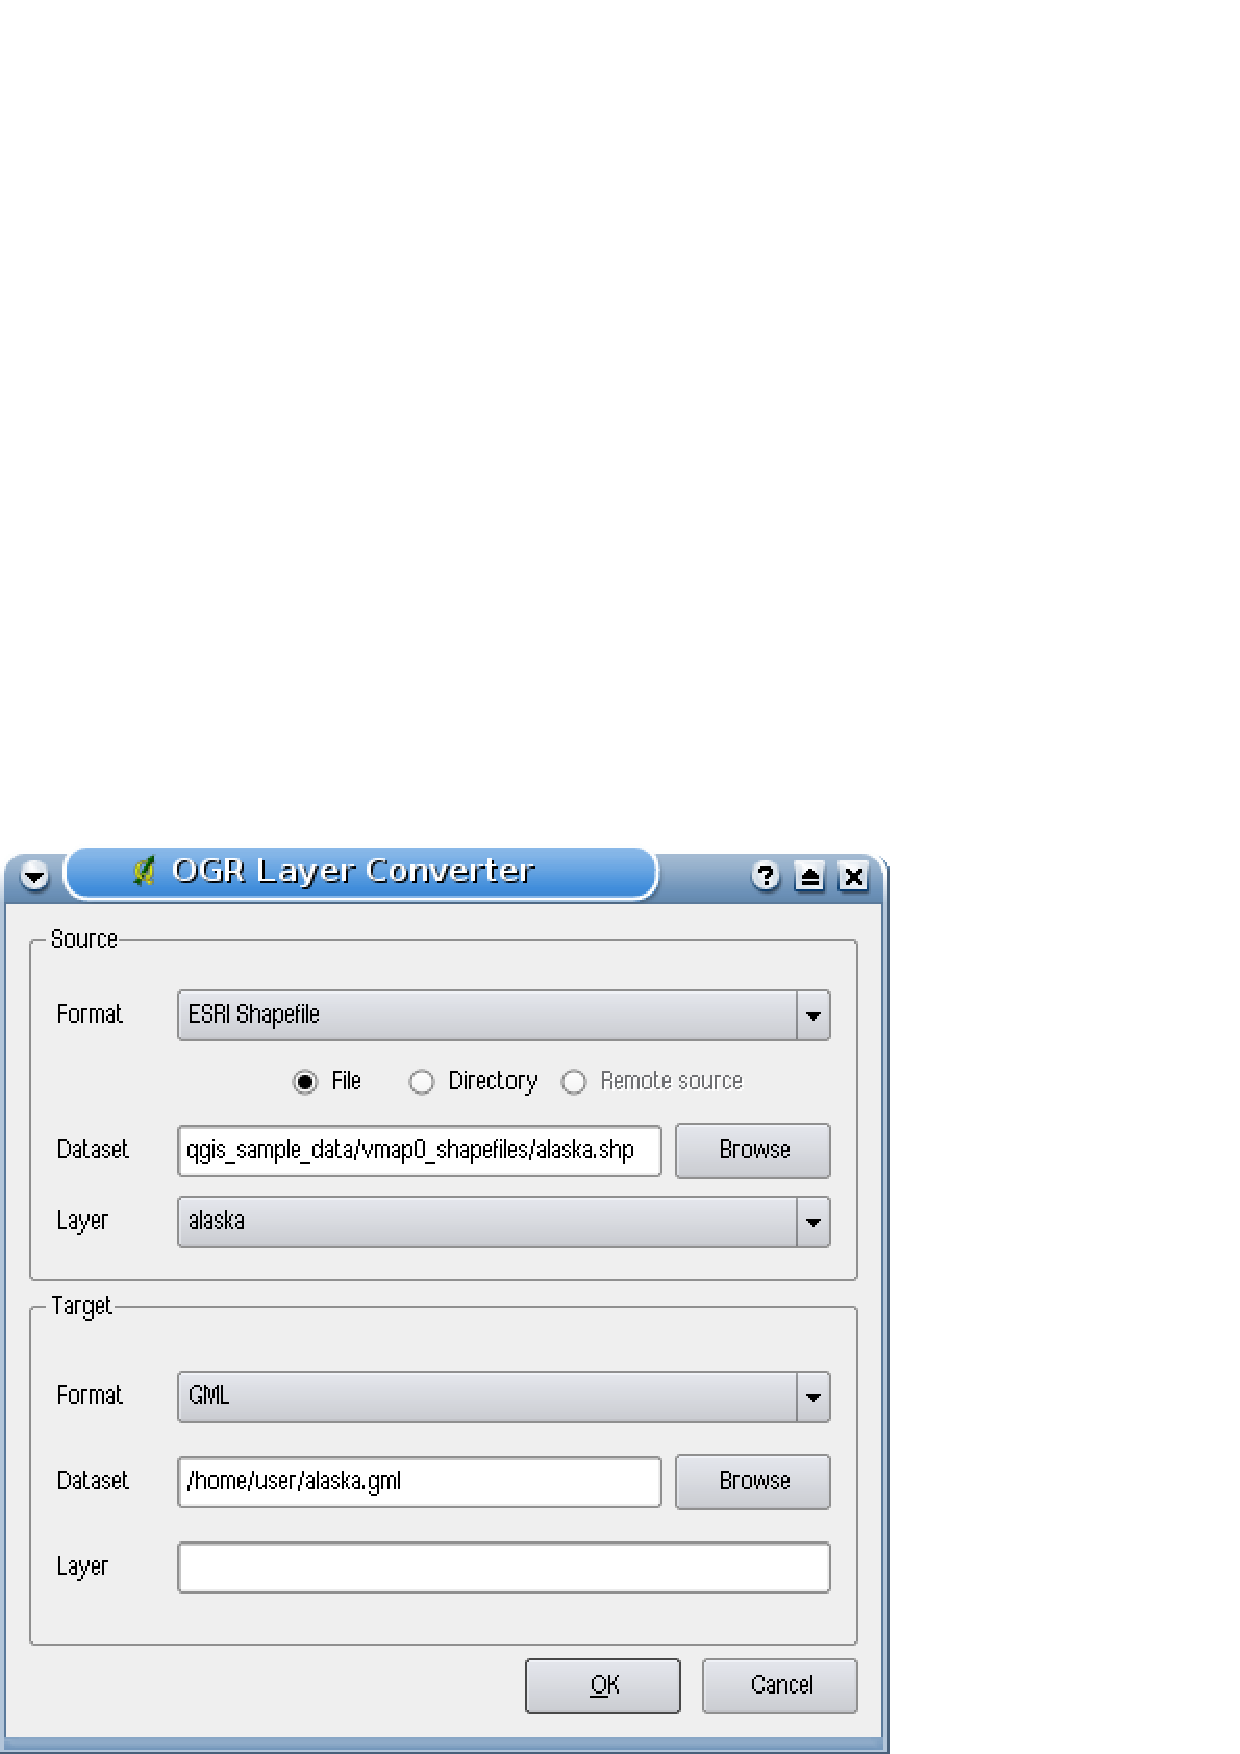
\includegraphics[clip=true, width=9cm]{ogrconverter_dialog}
\end{center}  
\end{figure}

\begin{enumerate}
  \item lanciare QGIS, caricare il Plugin Convertitore Layer OGR nel Gestore dei Plugin (vedere Sezione 
  \ref{sec:load_core_plugin}) e premere il tasto \toolbtntwo{ogr_converter}{Convertitore Layer OGR} che appare nel menu della barra strumenti QGIS. Appare la finestra di dialogo del plugin Convertitore Layer OGR come mostrato in Figura \ref{fig:ogrconverter_dialog}.
  \item Selezionare il formato OGR supportato \selectstring{ESRI Shapefile}{\ldots} e il percorso per il file vettoriale di input \filename{alaska.shp} nell'area Sorgente.
  \item Selezionare il formato OGR supportato \selectstring{GML}{\ldots}, definire un percorso e il nome per il file vettoriale in output \filename{alaska.gml} nell'area destinazione.
  \item Premere \button{Ok}.
\end{enumerate}

\newpage
